\chapter{Jax Manipulator}
\label{chap:metod}
A ativiade que tem como foco o uso de robôs manipuladores foi Jax Maninpulators. O oabjetivo dest ativadidade foi execução tarefa completamente autônoma. A tarefa consistia, primeiramente, na busca identificação de uma Tag que estava presente no ambiente de operação, e posteriormente, na execução de uma tarefa de movimentação do robô até uma  ação desejada. A ação deseja era a realização de um botão que também estava presente no ambiente.


%escrever oq sera apresentado

\subsection{Arquitetura Geral}
 A arquitetura geral, apresentada na Figura \ref{fig:Arquitetura geral}, relaciona de modo geral a interface do usuário, com a central de gerenciamento do sistema e com a interface com hardware. Neste contexto, no epectros de softwares  ,foi usado o sistema operacioanl Ubuntu 20.04, o midleware ROS2 Foxy  e pacote de softwate Moveit2. Para o sensorimaebti fora suados os encordes que estavam presentes dos servomotores Dynamixel e um câmera digital. Os servomotores dynamixel compôs o sistema mecânico do robô.  A alimentação dos sistema foi uma fonte 24 v.

 \begin{figure} [h!]	
    \centering

    \caption{Arquitetura Geral}
    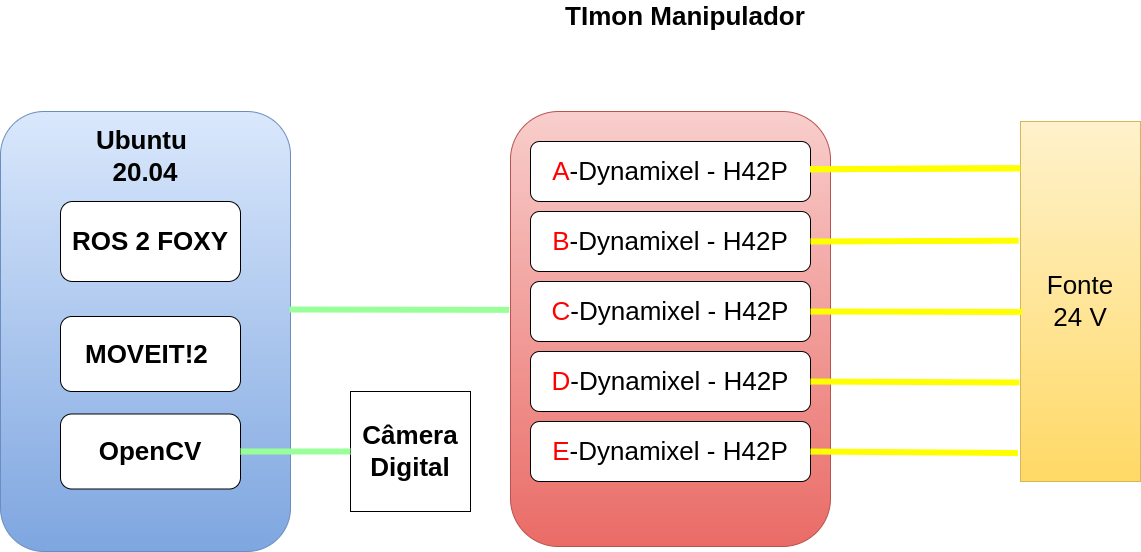
\includegraphics[width=0.8\textwidth]{system_architeture2.png}
    \caption*{Fonte: Autoria própria.}
    \label{fig:Arquitetura geral}
\end{figure}	


\subsection{Prototype Breakdown Structure}

Uma outra forma de apresentar a estrutura que foi usado é pelo  Prototype breakdown structure (PBS). O PBS ilustra os elementos que foram usados para a construção do sistemas.




\begin{figure} [h!]	
    \centering

    \caption{Arquitetura Geral}
    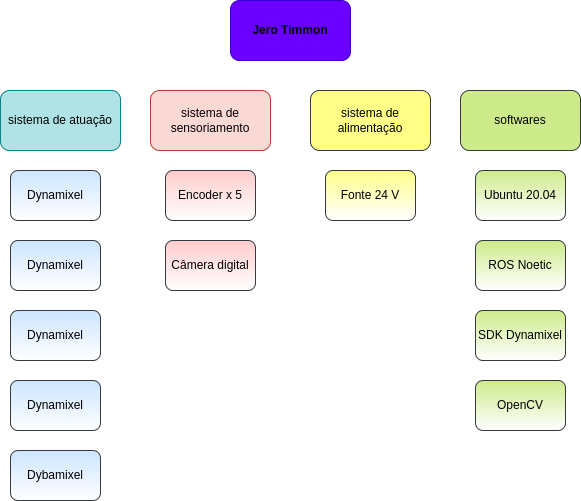
\includegraphics[width=0.8\textwidth]{pbs.png}
    \caption*{Fonte: Autoria própria.}
    \label{fig:PBS}
\end{figure}	
% %--------- NEW SECTION ----------------------
% \section{Interface do Usuário}
% \label{sec:ui}
% \lipsum[1]

% %--------- NEW SECTION ----------------------
% \section{Simulação do sistema}
% \label{sec:sim}
% \lipsum[2-4]

\subsection{Resultados}

Esta ativadidade conseguiu obter sucessos sobre o seu objetivo. O sistema foi capaz de executar a tarefa de forma completamente autônoma. Foi elaborado uma máquina de estados usando a linguagem de programação C++ para facilitar a exeução da tarefa.